% AutoKaggle system architecture.
% Build: pdflatex architecture.tex && pdftocairo -svg architecture.pdf architecture.svg
\documentclass[tikz,border=8pt]{standalone}
\usepackage[scaled]{helvet}
\renewcommand\familydefault{\sfdefault}
\usepackage[T1]{fontenc}
\usepackage{amssymb}
\usetikzlibrary{positioning,fit,backgrounds,arrows.meta,calc}

% Palette
\definecolor{ink}{HTML}{1F2937}
\definecolor{muted}{HTML}{6B7280}
\definecolor{stageC}{HTML}{2563EB}
\definecolor{agentC}{HTML}{7C3AED}
\definecolor{toolC}{HTML}{0F766E}
\definecolor{svcC}{HTML}{475569}
\definecolor{humanC}{HTML}{C2410C}
\definecolor{loopC}{HTML}{D97706}
\definecolor{execC}{HTML}{334155}
\definecolor{guardC}{HTML}{B91C1C}

\tikzset{
  every node/.style={font=\footnotesize, text=ink},
  panel/.style={draw=#1!55, fill=#1!5, rounded corners=4pt, line width=0.6pt},
  ptitle/.style={font=\footnotesize\bfseries, text=#1!80!black, anchor=north west},
  chip/.style={draw=#1!70, fill=white, rounded corners=2.5pt, line width=0.5pt,
               minimum height=0.78cm, align=center, font=\scriptsize, inner sep=2pt},
  box/.style={draw=#1!70, fill=#1!6, rounded corners=3pt, line width=0.6pt,
              align=center, inner sep=4pt},
  flow/.style={-{Stealth[length=2.2mm]}, line width=0.6pt, draw=muted},
  biflow/.style={{Stealth[length=2.2mm]}-{Stealth[length=2.2mm]}, line width=0.6pt, draw=muted},
  lbl/.style={font=\scriptsize\itshape, text=muted, fill=white, inner sep=1.5pt},
  later/.style={font=\tiny, text=muted},
}

\newcommand{\sub}[1]{\\[-1pt]{\tiny\color{muted}#1}}

\begin{document}
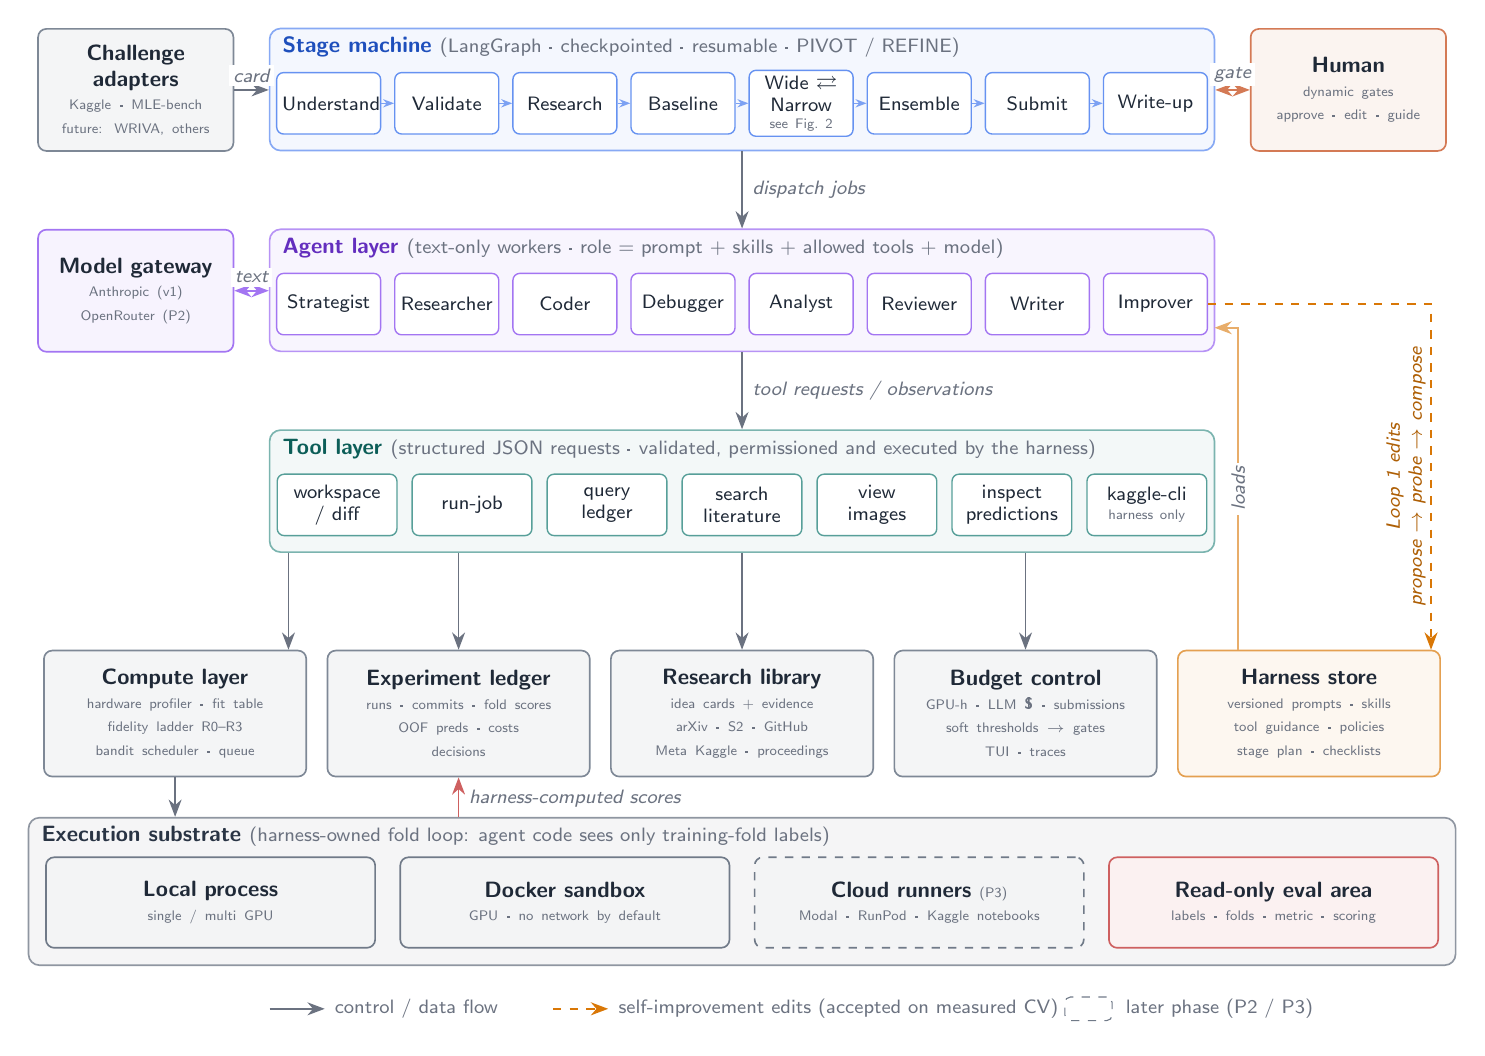
\begin{tikzpicture}

% ---------------- Band A: stage machine ----------------
\def\yA{0}
\foreach \name [count=\i from 0] in {Understand,Validate,Research,Baseline,{Wide $\rightleftarrows$ Narrow\\[-2pt]{\tiny\color{muted}see Fig.~2}},Ensemble,Submit,Write-up}{
  \node[chip=stageC, text width=1.18cm] (s\i) at (3.75+\i*1.5,\yA) {\name};
}
\foreach \i [evaluate=\i as \j using int(\i+1)] in {0,...,6}{
  \draw[-{Stealth[length=1.4mm]}, draw=stageC!60, line width=0.5pt] (s\i.east) -- (s\j.west);
}
\begin{scope}[on background layer]
  \node[panel=stageC, fit={(3,\yA+0.95) (15,\yA-0.6)}, inner sep=0pt] (stagepanel) {};
\end{scope}
\node[ptitle=stageC] at (stagepanel.north west) {\,Stage machine \textnormal{\textcolor{muted}{\scriptsize(LangGraph · checkpointed · resumable · PIVOT / REFINE)}}};

% Adapters (left) and human (right)
\node[box=svcC, text width=2.2cm, minimum height=1.55cm] (adapters) at (1.3,\yA+0.17)
  {\textbf{Challenge adapters}\sub{Kaggle · MLE-bench}\sub{future: WRIVA, others}};
\node[box=humanC, text width=2.2cm, minimum height=1.55cm] (human) at (16.7,\yA+0.17)
  {\textbf{Human}\sub{dynamic gates}\sub{approve · edit · guide}};

\draw[flow] (adapters.east) -- node[lbl, above=1pt] {card} (stagepanel.west |- adapters.east);
\draw[biflow, draw=humanC!70] (stagepanel.east |- human.west) -- node[lbl, above=1pt] {gate} (human.west);

% ---------------- Band B: agent layer ----------------
\def\yB{-2.55}
\foreach \name [count=\i from 0] in {Strategist,Researcher,Coder,Debugger,Analyst,Reviewer,Writer,Improver}{
  \node[chip=agentC, text width=1.18cm] (a\i) at (3.75+\i*1.5,\yB) {\name};
}
\begin{scope}[on background layer]
  \node[panel=agentC, fit={(3,\yB+0.95) (15,\yB-0.6)}, inner sep=0pt] (agentpanel) {};
\end{scope}
\node[ptitle=agentC] at (agentpanel.north west) {\,Agent layer \textnormal{\textcolor{muted}{\scriptsize(text-only workers · role = prompt + skills + allowed tools + model)}}};

\node[box=agentC, text width=2.2cm, minimum height=1.55cm] (gateway) at (1.3,\yB+0.17)
  {\textbf{Model gateway}\sub{Anthropic (v1)}\sub{OpenRouter (P2)}};
\draw[biflow, draw=agentC!70] (gateway.east) -- node[lbl, above=1pt] {text} (agentpanel.west |- gateway.east);

\draw[flow] (stagepanel.south) -- node[lbl, right=2pt] {dispatch jobs} (agentpanel.north);

% ---------------- Band C: tool layer ----------------
\def\yC{-5.1}
\foreach \name [count=\i from 0] in {workspace\\/ diff,run-job,query\\ledger,search\\literature,view\\images,inspect\\predictions,kaggle-cli\sub{harness only}}{
  \node[chip=toolC, text width=1.38cm] (t\i) at (3.857+\i*1.714,\yC) {\name};
}
\begin{scope}[on background layer]
  \node[panel=toolC, fit={(3,\yC+0.95) (15,\yC-0.6)}, inner sep=0pt] (toolpanel) {};
\end{scope}
\node[ptitle=toolC] at (toolpanel.north west) {\,Tool layer \textnormal{\textcolor{muted}{\scriptsize(structured JSON requests · validated, permissioned and executed by the harness)}}};

\draw[flow] (agentpanel.south) -- node[lbl, right=2pt] {tool requests / observations} (toolpanel.north);

% ---------------- Band D: core services ----------------
\def\yD{-7.75}
\node[box=svcC, text width=3.05cm, minimum height=1.6cm] (compute) at (1.8,\yD)
  {\textbf{Compute layer}\sub{hardware profiler · fit table}\sub{fidelity ladder R0–R3}\sub{bandit scheduler · queue}};
\node[box=svcC, text width=3.05cm, minimum height=1.6cm] (ledger) at (5.4,\yD)
  {\textbf{Experiment ledger}\sub{runs · commits · fold scores}\sub{OOF preds · costs}\sub{decisions}};
\node[box=svcC, text width=3.05cm, minimum height=1.6cm] (library) at (9.0,\yD)
  {\textbf{Research library}\sub{idea cards + evidence}\sub{arXiv · S2 · GitHub}\sub{Meta Kaggle · proceedings}};
\node[box=svcC, text width=3.05cm, minimum height=1.6cm] (budget) at (12.6,\yD)
  {\textbf{Budget control}\sub{GPU-h · LLM \$ · submissions}\sub{soft thresholds $\rightarrow$ gates}\sub{TUI · traces}};
\node[box=loopC, text width=3.05cm, minimum height=1.6cm] (store) at (16.2,\yD)
  {\textbf{Harness store}\sub{versioned prompts · skills}\sub{tool guidance · policies}\sub{stage plan · checklists}};

\foreach \n in {ledger,library,budget}{
  \draw[flow] (toolpanel.south -| \n.north) -- (\n.north);
}
% compute sits partly outside the tool panel, so its arrow leaves the panel's left edge
\coordinate (cp0) at ($(toolpanel.south west)+(0.25,0)$);
\draw[flow] (cp0) -- (cp0 |- compute.north);

% ---------------- Band E: execution substrate ----------------
\def\yE{-10.15}
\node[box=execC, text width=3.9cm, minimum height=1.15cm] (local) at (2.25,\yE)
  {\textbf{Local process}\sub{single / multi GPU}};
\node[box=execC, text width=3.9cm, minimum height=1.15cm] (docker) at (6.75,\yE)
  {\textbf{Docker sandbox}\sub{GPU · no network by default}};
\node[box=execC, text width=3.9cm, minimum height=1.15cm, dashed] (cloud) at (11.25,\yE)
  {\textbf{Cloud runners} {\tiny\color{muted}(P3)}\sub{Modal · RunPod · Kaggle notebooks}};
\node[box=guardC, text width=3.9cm, minimum height=1.15cm] (guard) at (15.75,\yE)
  {\textbf{Read-only eval area}\sub{labels · folds · metric · scoring}};

\begin{scope}[on background layer]
  \node[panel=execC, fit={(local)(guard)}, inner sep=6pt, yshift=4pt, inner ysep=10pt] (execpanel) {};
\end{scope}
\node[ptitle=execC] at (execpanel.north west) {\,Execution substrate \textnormal{\textcolor{muted}{\scriptsize(harness-owned fold loop: agent code sees only training-fold labels)}}};

\draw[flow] (compute.south) -- (compute.south |- execpanel.north);

% scores flow from read-only area to ledger
\draw[flow, draw=guardC!70] (execpanel.north -| ledger.south) ++(0,0) -- (ledger.south)
  node[lbl, pos=0.45, right=2pt] {harness-computed scores};

% ---------------- Self-improvement loop (right column) ----------------
\coordinate (rc) at (17.75,0);
\draw[-{Stealth[length=2.2mm]}, draw=loopC, line width=0.8pt, dashed]
  (a7.east) -- (a7.east -| rc) -- (rc |- store.north)
  node[pos=0.5, lbl, text=loopC!80!black, align=center, rotate=90, anchor=south] {Loop 1 edits\\propose $\rightarrow$ probe $\rightarrow$ compose};
\coordinate (ld0) at ($(store.north)+(-0.9,0)$);
\coordinate (ld1) at (ld0 |- 0,\yB-0.3);
\draw[-{Stealth[length=2.2mm]}, draw=loopC!60, line width=0.6pt]
  (ld0) -- node[lbl, pos=0.5, rotate=90] {loads} (ld1) -- (15,\yB-0.3);

% ---------------- Legend ----------------
\def\yL{-11.5}
\draw[flow] (3.0,\yL) -- ++(0.7,0) node[right, font=\scriptsize, text=muted] {control / data flow};
\draw[-{Stealth[length=2.2mm]}, draw=loopC, line width=0.8pt, dashed] (6.6,\yL) -- ++(0.7,0)
  node[right, font=\scriptsize, text=muted] {self-improvement edits (accepted on measured CV)};
\node[draw=execC!70, dashed, rounded corners=2pt, minimum width=0.6cm, minimum height=0.3cm] at (13.4,\yL) {};
\node[right, font=\scriptsize, text=muted] at (13.75,\yL) {later phase (P2 / P3)};

\end{tikzpicture}
\end{document}
